\documentclass{ctexbook}

% Bookmark

\usepackage{bookmark}

% Figure

\usepackage{amsmath, amssymb, pgfplots}
\pgfplotsset{compat = newest, width = 6cm}

% Caption

\usepackage[labelsep = space]{caption}
\renewcommand{\thefigure}{\thechapter.\arabic{figure}~}
\renewcommand{\thetable}{\thechapter.\arabic{table}~}
\DeclareCaptionFont{kaishu}{\kaishu}
\captionsetup{font = kaishu}

% Table 

\usepackage{multirow, float}
\renewcommand{\arraystretch}{1.5}

% Font

\usepackage{textcomp, mathcomp, bm}

\usepackage{graphicx}
\usepackage{ctex}
\xeCJKsetup{CJKmath = true}
\usepackage{amsmath}
\usepackage[top=2cm, bottom=2cm, left=3cm, right=3cm]{geometry}
\usepackage{setspace}
\usepackage{titlesec}
\usepackage{hyperref}
\usepackage{fancyhdr}
\usepackage{draftwatermark}
\SetWatermarkText{}
% \SetWatermarkLightness{0.95}
% \SetWatermarkScale{1}
\renewcommand{\headrulewidth}{0pt}
\fancyhf{}
\fancyhead{}
\fancyfoot[C]{\thepage}
\pagestyle{fancy}

\def\blue#1{{\bf\color{blue}#1}}
\def\red#1{{\bf\color{red}#1}}
\def\mathline#1{{\red{\begin{equation}\bm{#1}\end{equation}}}}
\def\titlename#1{\caption{#1}\label{#1}}

\title{\huge\textbf{中学物理}}
\author{田怿}
\date{\today}

\begin{document}

\maketitle
\thispagestyle{empty}

\ctexset{
	chapter={name={Part~,},number=\Roman{chapter}},
	section={number=\arabic{section}},
	subsection={number=\arabic{section}.\arabic{subsection}},
}
\tableofcontents
\setcounter{page}{0}
\thispagestyle{empty}

\setstretch{1.05}

\chapter{热学}

\newpage
{\bf 热学是研究物质\blue{热运动}规律及其应用的物理学分支.}

\section{分子动理论}

\subsection{分子动理论(molecular kinetic theory)}
\vspace{10pt}
\begin{itemize}
\item 物质是由大量分子组成的.
\item 分子在\blue{永不停息}地做\blue{无规则}运动.
\item 分子之间存在相互作用力.
\item 分子直径约为 \blue{$\bf10^{-10}m$}.
\item 18g 水中含有水分子的个数约为 \blue{$\bf6.02\times10^{23}$},即为阿伏伽德罗常数 $N_{\text{A}}$.
\item 在研究物体的热运动性质和规律时,不必区分它们在化学变化中所起的不同作用,而把组成物体的微粒统称为\blue{分子}(molecule).
\item 不同的物质在相互接触时\blue{自发地}彼此进入对方的现象叫做\blue{扩散}(diffusion).
\item 扩散现象可以发生在气体、液体和固体之间.
\item 扩散现象是物质分子永不停息地做无规则运动的证据之一.
\item 悬浮微粒的无规则运动叫做\blue{布朗运动}(Brownian motion).
\item \blue{悬浮微粒的无规则运动并不是分子的运动},但可以间接地反应液体分子运动的无规则性.
\item 分子的无规则运动叫做\blue{热运动}(thermal motion). 
\item \blue{温度}是\blue{分子热运动剧烈程度}的标志.
\item \blue{分子之间存在引力},\blue{分子之间存在斥力}.
\item 分子之间,引力和斥力\blue{同时存在}.
\item 分子间的作用力 $F$ 与分子间距离 $r$ 有关. 即:
\newline 当 $r=r_0$ 时,分子间的作用力 $F$ 为 0,这个位置被称为\blue{平衡位置}.
\newline 当 $r>r_0$ 时,分子间的作用力 $F$ 表现为引力.
\newline 当 $r<r_0$ 时,分子间的作用力 $F$ 表现为斥力.
\begin{figure}[H]
	\centering
	\begin{tikzpicture}
	\begin{axis}[
		axis lines = middle,
		xmin = 0, xmax = 8,
		ymin = -4, ymax = 4,
		smooth, thick,
		xlabel = {$r$}, ylabel = {$F$},
		xlabel style = {anchor = north},
		ylabel style = {anchor = east},
		xtick = {0.83627}, xticklabels = {$r_0$}, 
		ytick = \empty,
		samples = 200,
		legend entries = {\kaishu{引力}, \kaishu{斥力}},
		legend style = {font = \small},
	]
		\addplot+[no marks, domain = 0.5 : 7.5]{6 / (x + 1) ^ 1.3};
		\addplot+[no marks, domain = 0.5 : 7.5]{-5 / (x + 1)};
	\end{axis}
	\end{tikzpicture}
	~~
	\begin{tikzpicture}
	\begin{axis}[
		axis lines = middle,
		xmin = 0, xmax = 4,
		ymin = -2, ymax = 2,
		smooth, thick,
		xlabel = {$r$}, ylabel = {$F$},
		xlabel style = {anchor = north},
		ylabel style = {anchor = east},
		xtick = {0.46607}, xticklabels = {$r_0$}, xtick style = {anchor = north east},
		ytick = \empty,
		samples = 200,
		legend entries = {\kaishu{合力}},
		legend style = {font = \small},
	]
		\addplot+[no marks, domain = 0.25 : 3.75]{9 / ((x + 0.85) ^ 6) - 3 / ((x + 0.85) ^ 2)};
	\end{axis}
	\end{tikzpicture}
	\titlename{分子间的作用力与分子间的距离的关系}
\end{figure}
\end{itemize}

\subsection{固体~~液体~~气体}
\vspace{10pt}
\begin{itemize}
\item 固体分子间的距离小,不容易被压缩和拉伸,具有一定的体积和形状.
\item 气体分子间的距离很大,彼此间几乎没有作用力. 具有流动性,容易被压缩.
\item 液体分子间的距离比气体小、比固体大,液体分子间的作用力比固体小、比气体大,分子没有固定的位置,运动较自由. 液体较难被压缩,没有一定的形状,具有流动性.
\begin{table}[H]
	\kaishu
	\centering
	\begin{tabular}{ccccc}
	\toprule
	\multirow{2}*{物态} & \multicolumn{2}{c}{微观特性} & \multicolumn{2}{c}{宏观特性} \\
	& 分子间距离 & 分子间作用力 & 固定形状 & 固定体积 \\ 
	\midrule
	固态 & 很小 & 很大 & 是 & 是 \\ 
	液态 & 较大 & 较大 & 否 & 是 \\ 
	气态 & 很大 & 很小 & 否 & 否 \\ 
	\bottomrule
	\end{tabular}
	\titlename{固体~~液体~~气体}
\end{table}
\end{itemize}
\newpage
\section{内能}

\subsection{内能}
\vspace{10pt}
\begin{itemize}
\item 分子由于\blue{热运动}而具有的能叫做\blue{分子动能}.
\item 系统中所有分子的动能的平均值叫做\blue{分子热运动的平均动能}.
\item 物体温度升高时,分子热运动的平均动能增加.
\item \blue{温度}是\blue{分子热运动的平均动能}的标志.
\item 单原子分子的平均动能 $\overline{E_k}=\frac32kT$,即 $\overline{E_k}\propto T$.
\item 分子之间由于存在\blue{相互作用力}而具有的能叫做\blue{分子势能}.
\item 分子势能 $E_p$ 与分子间的距离 $r$ 有关. 即:
\newline 当 $r=r_0$ 时,分子间的作用力 $F$ 为 0,\blue{分子势能最小}.
\newline 当 $r>r_0$ 时,分子间的作用力 $F$ 表现为引力,分子势能减小.
\newline 当 $r<r_0$ 时,分子间的作用力 $F$ 表现为斥力,分子势能增大.
\item 分子势能的大小由\blue{分子间的相对位置}决定. 如果选定分子间距离 $r$ 为无穷远时的分子势能 $E_p$ 为 0,则分子势能 $E_p$ 随分子间距离变化的情况如图所示.
\begin{figure}[H]
	\centering
	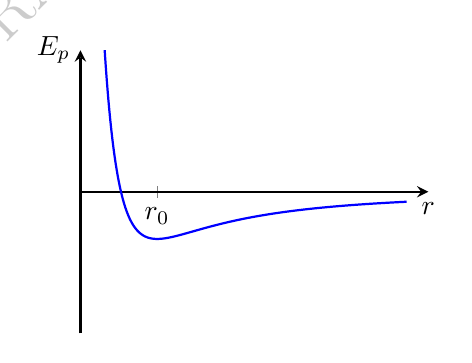
\begin{tikzpicture}
	\begin{axis}[
		axis lines = middle,
		xmin = 0, xmax = 4,
		ymin = -2, ymax = 2,
		smooth, thick,
		xlabel = {$r$}, ylabel = {$E_p$},
		xlabel style = {anchor = north},
		ylabel style = {anchor = east},
		xtick = {0.88205}, xticklabels = {$r_0$}, xtick style = {anchor = north east},
		ytick = \empty,
		samples = 200,
	]
		\addplot+[no marks, domain = 0.25 : 3.75]{9 / ((x + 0.85) ^ 6) - 3 / ((x + 0.85) ^ 2)};
	\end{axis}
	\end{tikzpicture}
	\titlename{分子势能与分子间的距离的关系}
\end{figure}
\item 分子势能与物体体积有关.
\item 物体中所有分子的\blue{分子动能与分子势能的总和},叫做物体的\blue{内能}(internal energy). 任何物体都具有内能. 内能的单位是\blue{焦耳($\bf J$)}.
\item 物体的内能与\blue{温度}和\blue{体积}有关.
\end{itemize}

\newpage
\subsection{比热容}
\vspace{10pt}
\begin{itemize}
\item 内能由\blue{高温}物体转移到\blue{低温}物体的过程叫做\blue{热传递}.
\item 热传递的基本方式包括传导、对流和辐射.
\item 在热传递过程中,传递能量的多少叫做\blue{热量}(quantityo of heat). 用符号 \blue{$\bf{\it Q}$} 表示. 单位是\blue{焦耳}. 
\item 物体吸收热量是内能增加,放出热量时内能减少. \blue{热量是物体内能改变的量度}.
\item 一定质量的某种物体,在温度升高(或降低)时吸收(或放出)的热量与它的质量和升高(或降低)的温度乘积之比,叫做这种物质的\blue{比热容}(specific heat capacity). 用符号 \blue{$c$} 表示. 单位是\blue{焦每千克摄氏度($\bf J/(kg\cdot\textcelsius)$)}. 有:
\mathline{c=\frac{\Delta Q}{m\Delta t}}
\item 比热容反映\blue{物质自身性质}的物理量.
\item 不同的物质,比热容一般不同.
\item 水的比热容为 \blue{$\bf4.2\times10^3J/(kg\cdot\textcelsius)$}.
\item 热量的计算有 \blue{$\Delta Q=cm\Delta t$}.
\item \blue{热平衡方程},即 \blue{$\Delta_吸=\Delta_放$}.
\end{itemize}
\newpage
\section{热机}

\subsection{热机}
\vspace{10pt}
\begin{itemize}
\item \blue{热机}(heat engine),即利用内能做功(\blue{内能转化为机械能})的机械.
\item \blue{蒸汽机},即利用水蒸气膨胀做功的热机. 蒸汽机属于外燃机.
\item 活塞从气缸的一端运动到另一端的过程叫做一个\blue{冲程}.
\item 四冲程汽油机一般包括\blue{吸气}、\blue{压缩}、\blue{做功}和\blue{排气}四个冲程.
\item \blue{汽油机}和\blue{柴油机}都属于\blue{内燃机}.
\item \blue{汽轮机}和\blue{喷气发动机}.
\end{itemize}
\newpage
\section{热力学定律}

\vspace{10pt}
\begin{itemize}
\item 热学包括\blue{热力学}和\blue{统计物理}.
\item 热力学的研究对象叫做\blue{热力学系统}(thermodynamic system),简称\blue{系统}. 热力学系统是由大量分子组成的.
\item 系统之外与系统发生相互作用的其他物体统称为\blue{外界}.
\end{itemize}

\subsection{系统内能的改变}
\vspace{10pt}
\begin{itemize}
\item 改变系统内能的两种方式是\blue{热传递}和\blue{做功}.
\item 在热传递过程中,系统吸收热量内能增加,放出热量内能减少.
\item 热量是\blue{热传递过程中}系统内能变化的量度.
\item 系统与外界没有热传递的过程叫做\blue{绝热过程}(adiabatic process).
\item 在绝热过程中,外界对系统做功,系统内能增加;系统对外界做功,系统内能减少.
\item 做功是\blue{绝热过程中}系统内能变化的量度.
\item 焦耳的实验表明\blue{热传递和做功对改变系统的内能是等效的}.
\end{itemize}

\subsection{热力学第一定律}
\vspace{10pt}
\begin{itemize}
\item \blue{热力学第一定律}(first law of thermodynamics),即热力学系统内能 $U$ 的变化量等于系统从外界吸收的热量(系统向外界放出的热量)与外界对系统做的功(系统对外界做的功)之和. 有:
\mathline{\Delta U=Q+W}
\newline 系统对外界吸热,$Q$ 为正值;系统对外界放热,$Q$ 取负值;外界对系统做功,$W$ 取正值;系统对外界做功,$W$ 取负值.
\end{itemize}

\subsection{能量守恒定律}
\vspace{10pt}
\begin{itemize}
\item 不同形式的能量可以在一定条件下相互转化.
\item \blue{能量守恒定律}(law of conservation of energy),即能量既不会凭空产生,也不会凭空消失,它只能从一种形式\blue{转化}为其他形式,或者从一个物体\blue{转移}到其他物体,在转化或转移的过程中,能量的总量保持不变.
\item 能量守恒定律是自然界最普遍、最重要的基本定律之一.
\item 能量守恒定律的本质是\blue{时间平移对称性}.
\item \blue{永动机},即不需要动力就能源源不断地对外做功的机器,分为第一类永动机和第二类永动机.
\item 能量守恒定律的另一种表述为\blue{第一类永动机不可能制成}.
\end{itemize}

\subsection{热力学第二定律}
\vspace{10pt}
\begin{itemize}
\item 一切与热现象有关的宏观自然过程都是\blue{不可逆}的.
\item \blue{热力学第二定律}(second law of thermodynamics).
\item \blue{克劳修斯表述},即热量不能\blue{自发}地从低温物体传到高温物体. 自发是指不需要任何第三者的介入,不会对任何第三者产生任何影响. 自发的方向是从高温物体指向低温物体.
\item 克劳修斯表述阐述了\blue{传热的方向性}.
\item \blue{开尔文表述},即\blue{不可能从单一热库吸收热量},使之完全变成功,而不产生其他影响. 不可能从单一热库吸热,而且一定会向另一个热库放热.
\item 开尔文表述阐述了\blue{机械能与内能转化的方向性}.
\item \blue{热力学第二定理的另一种表述为}\blue{第二类永动机不可能制成}.
\item 热力学第二定律的克劳修斯表述和开尔文表述是\blue{等价的}.
\item \blue{能量耗散},即不同形式的能量最终都转化为\blue{内能}并分散在环境中的过程.
\end{itemize}


\end{document}